\documentclass[11pt,a4paper]{article}
\usepackage[T1]{fontenc}
\usepackage[utf8]{inputenc}
\usepackage[polish]{babel}
\usepackage{amsmath}
\usepackage[margin=1.8cm]{geometry}
\usepackage{graphicx}
\usepackage{enumitem}
\usepackage{xcolor}
\usepackage{parskip}

\setlist[itemize]{leftmargin=1.3em,itemsep=2pt,topsep=2pt}
\newcommand{\obs}[1]{\textcolor{gray!30!black}{#1}}
\pagestyle{empty}

\begin{document}

{\Large\bfseries Analiza wydajności \texttt{heat3d} (stencil dyfuzji ciepła 3D, Chapel)}\par
\vspace{2pt}
{\small Klaster obliczeniowy, conduit GASNet. \textbf{Locale} w Chapelu to \textbf{osobny proces}
(z własną pamięcią), uruchamiany flagą \texttt{-nl N}; w tych testach jeden locale na węzeł fizyczny.
Liczbę \emph{wątków wewnątrz jednego locale} steruje \texttt{CHPL\_RT\_NUM\_THREADS\_PER\_LOCALE} --
to dwie niezależne osie zrównoleglenia (locale = między procesami, wątki = w obrębie procesu). Lewy
panel każdego rysunku: rozkład czasu wykonania (box-plot, ${\sim}10$ przebiegów/konfigurację; czerwona
linia -- mediana, zielony diament -- średnia, ,,najszybszy'' -- najniższa mediana). Prawy panel:
metryka pochodna.}\par
\vspace{6pt}
\hrule
\vspace{10pt}

%============================================================
\noindent{\large\bfseries 1. Skalowanie po węzłach} \quad {\small($1000^3$, stała liczba wątków)}\par
\vspace{4pt}
\begin{minipage}[t]{0.60\textwidth}
  \vspace{0pt}
  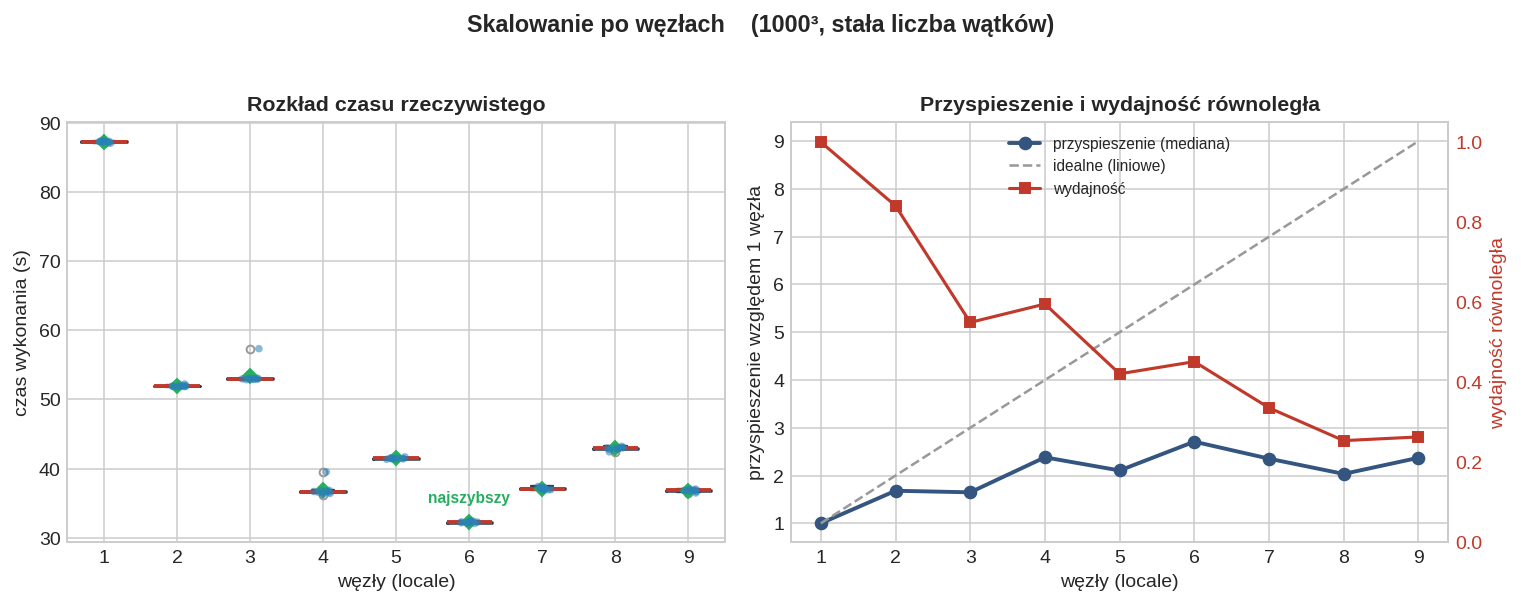
\includegraphics[width=\linewidth]{node_scaling.png}
\end{minipage}\hfill
\begin{minipage}[t]{0.37\textwidth}
  \vspace{0pt}
  \small
  \begin{itemize}
    \item Czas spada z ${\sim}87$\,s (1 węzeł) do minimum \textbf{${\sim}32$\,s przy 6 węzłach} i dalej
          \textbf{nie maleje} (7--10 węzłów: ${\sim}37$\,s).
    \item Silny ,,ząbek piły'' (parzysta/nieparzysta liczba węzłów) -- podział $1000^3$ na nierówne
          płaty daje różne obciążenia i różną liczbę bajtów/krok.
    \item Przyspieszenie płaszczy się na \textbf{${\sim}2{,}4\times$}, mocno poniżej idealnej prostej;
          wydajność równoległa spada do \textbf{${\sim}0{,}24$} przy 10 węzłach.
    \item \textbf{Wniosek:} aplikacja jest ograniczona komunikacją (\emph{comm-bound}) -- wymiana halo
          (\texttt{updateFluff}) rośnie liniowo z liczbą węzłów, a wolny conduit zjada zysk z rdzeni.
  \end{itemize}
\end{minipage}
\vspace{10pt}
\hrule
\vspace{10pt}

%============================================================
\noindent{\large\bfseries 2. Skalowanie rozmiaru sześcianu} \quad {\small(9 węzłów)}\par
\vspace{4pt}
\begin{minipage}[t]{0.60\textwidth}
  \vspace{0pt}
  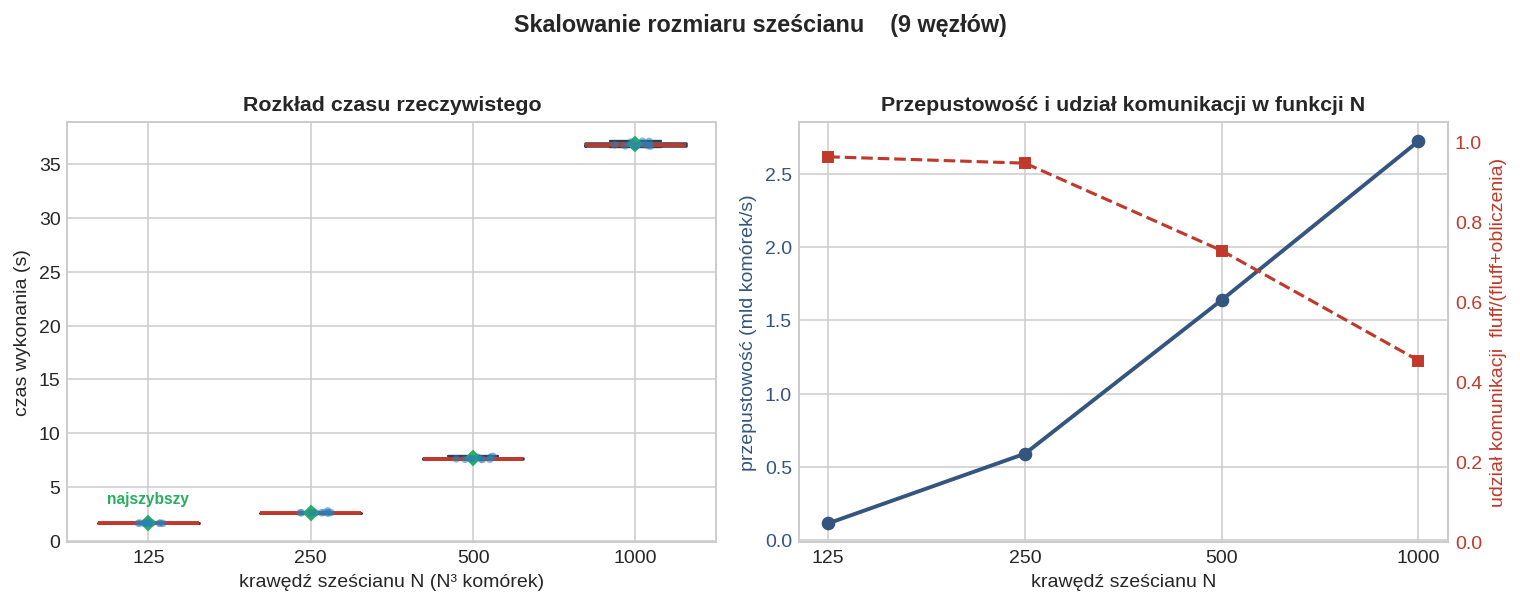
\includegraphics[width=\linewidth]{cube_size.png}
\end{minipage}\hfill
\begin{minipage}[t]{0.37\textwidth}
  \vspace{0pt}
  \small
  \begin{itemize}
    \item Czas rośnie ${\sim}$sześciennie z krawędzią $N$ ($N^3$ komórek): od ${\sim}1{,}7$\,s ($125^3$)
          do ${\sim}220$\,s ($2000^3$).
    \item Przepustowość rośnie z $0{,}12$ do \textbf{${\sim}3{,}6$ Gkom./s} (miliardów aktualizacji
          komórek na sekundę).
    \item Udział komunikacji \texttt{fluff/(fluff+obliczenia)} spada z \textbf{$0{,}96$ do $0{,}28$}.
    \item \textbf{Wniosek:} odwrotność rys.\,1 -- większy sześcian to korzystniejszy stosunek obliczeń
          do komunikacji (objętość $N^3$ rośnie szybciej niż powierzchnia halo $N^2$). Małe siatki są
          zdominowane przez sieć i marnują klaster.
    \item \emph{Uwaga:} przy $2000^3$ tylko 2 realne przebiegi (reszta dopełniona średnią).
  \end{itemize}
\end{minipage}
\vspace{10pt}
\hrule
\vspace{10pt}

%============================================================
\noindent{\large\bfseries 3. Skalowanie wątków przy 9 locale} \quad {\small($1000^3$, 100 kroków)}\par
\vspace{4pt}
\begin{minipage}[t]{0.60\textwidth}
  \vspace{0pt}
  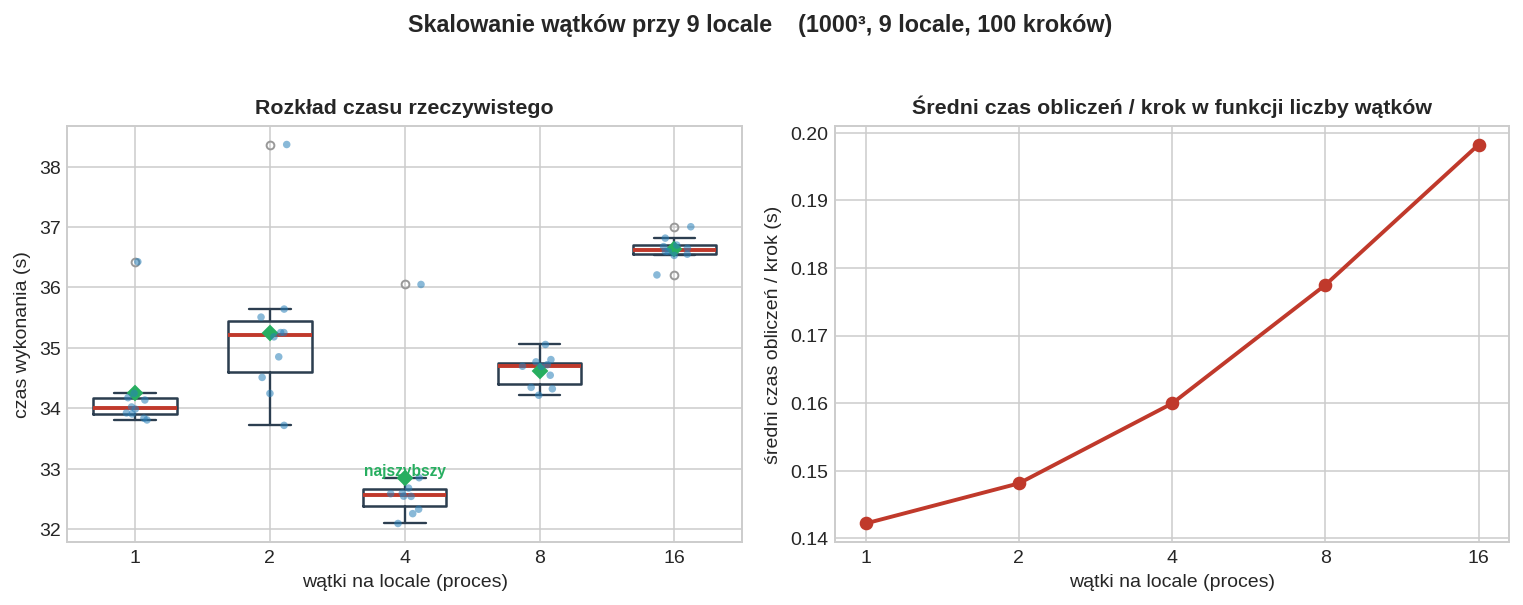
\includegraphics[width=\linewidth]{threads_9nodes.png}
\end{minipage}\hfill
\begin{minipage}[t]{0.37\textwidth}
  \vspace{0pt}
  \small
  \begin{itemize}
    \item Stałe \textbf{9 locale} (9 procesów, po jednym na węzeł); zmienną jest liczba \emph{wątków
          w obrębie każdego locale} ($1 \to 16$).
    \item Czas niemal płaski (${\sim}33$--$37$\,s); minimum przy \textbf{4 wątkach/locale}
          (${\sim}32{,}6$\,s), potem rośnie.
    \item Średni czas obliczeń \emph{na krok} rośnie monotonicznie z liczbą wątków
          ($0{,}14 \to 0{,}20$\,s).
    \item \textbf{Wniosek:} dokładanie wątków w obrębie procesu nie pomaga -- problem jest
          \emph{comm-bound} (wymiana halo między locale, nie moc obliczeniowa). Wzrost czasu
          obliczeń/krok to nadsubskrypcja rdzeni: rywalizacja o pasmo pamięci i o wątek pollujący
          GASNet, który już zajmuje jeden rdzeń w każdym procesie.
  \end{itemize}
\end{minipage}
\vspace{10pt}
\hrule
\vspace{10pt}

%============================================================
\noindent{\large\bfseries 4. Skalowanie wątków w obrębie jednego locale} \quad {\small($1000^3$, 10 kroków)}\par
\vspace{4pt}
\begin{minipage}[t]{0.60\textwidth}
  \vspace{0pt}
  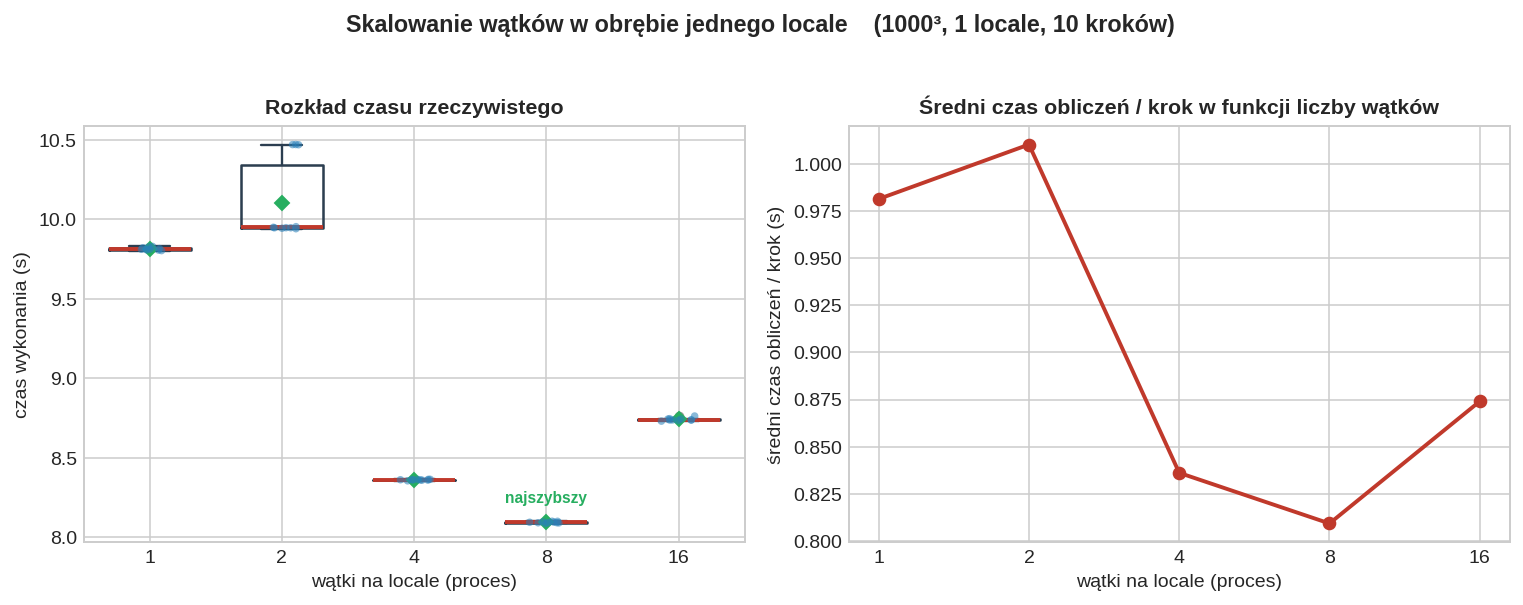
\includegraphics[width=\linewidth]{threads_1node.png}
\end{minipage}\hfill
\begin{minipage}[t]{0.37\textwidth}
  \vspace{0pt}
  \small
  \begin{itemize}
    \item Próba kontrolna: \textbf{1 locale} (1 proces), więc \textbf{brak komunikacji między
          procesami} -- wymiana halo jest lokalna/pomijalna. Izoluje sam narzut wątków.
    \item Wyraźne minimum przy \textbf{8 wątkach} (${\sim}8{,}1$\,s wobec $9{,}8$\,s dla 1 wątku).
    \item Czas obliczeń/krok \textbf{spada} dla 1$\to$8 wątków ($0{,}98 \to 0{,}81$\,s), potem lekko
          rośnie przy 16 (nadsubskrypcja ponad liczbę rdzeni fizycznych).
    \item \textbf{Wniosek:} w obrębie pojedynczego procesu jądro obliczeniowe skaluje się wątkami
          poprawnie. Potwierdza to, że słabe skalowanie z rys.\,3 wynika z komunikacji między locale
          (sieć), a nie z kodu obliczeniowego.
  \end{itemize}
\end{minipage}
\vspace{10pt}
\hrule
\vspace{10pt}

%============================================================
\noindent{\large\bfseries 5. Skalowanie wątków, $1000^3$ na węźle .13} \quad {\small(1 locale, Chapel 2.9 mpi-conduit, 10 kroków)}\par
\vspace{4pt}
\begin{minipage}[t]{0.60\textwidth}
  \vspace{0pt}
  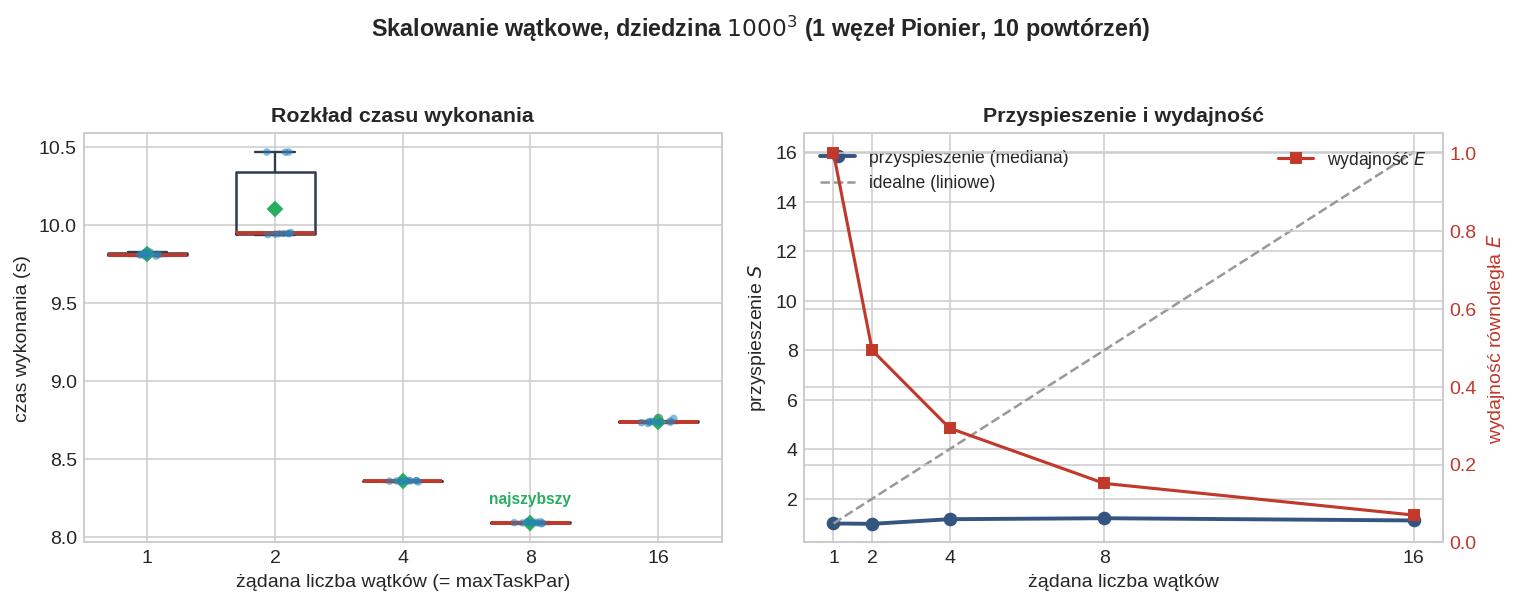
\includegraphics[width=\linewidth]{threads_1000.png}
\end{minipage}\hfill
\begin{minipage}[t]{0.37\textwidth}
  \vspace{0pt}
  \small
  \begin{itemize}
    \item Powtórzenie rys.\,4 na dużej kostce i dedykowanym węźle .13 (24 rdzenie, 31\,GB, 0 swap).
          1 locale, zmienne wątki $1 \to 16$.
    \item Przy 24 rdzeniach \texttt{maxTaskPar} = wartości żądanej dla \emph{każdej} konfiguracji
          (brak ograniczania qthreads) -- widać to wprost w logu (\texttt{[cfg] ... maxTaskPar=}).
    \item Duży skok $1\to2$ wątki, minimum przy \textbf{4 wątkach} (${\sim}5{,}60$\,s), powyżej --
          wolniej.
    \item Przyspieszenie płaszczy się na \textbf{${\sim}1{,}55\times$}, mocno poniżej ideału;
          wydajność równoległa spada z $1{,}0$ do \textbf{${\sim}0{,}09$ przy 16 wątkach}.
    \item \textbf{Wniosek:} jądro jest \emph{ograniczone pasmem pamięci} -- powyżej 4 wątków dokładanie
          rdzeni nie pomaga (pasmo wysycone), a narzut synchronizacji/NUMA lekko pogarsza wynik.
          Kontrast z rys.\,4 ($500^3$, box 12-rdz.): tam za mało pracy na krok, więc 1 wątek był
          najszybszy; tu $8\times$ większa kostka amortyzuje narzut i optimum przypada na 4 wątki.
  \end{itemize}
\end{minipage}
\vspace{10pt}
\hrule
\vspace{8pt}

{\small\emph{Metodyka:} dla rys.\,1--4 liczba wątków nie jest zapisana w logach -- odtworzono ją
z kolejności czasowej przebiegów (segmentacja DP), więc etykiety 1/2/4/8/16 są dedukowane; rozmiar $N$
wyliczono z $\mathrm{round}(\sqrt[3]{\text{sum}})$, a liczba locale jest jedyną wartością zapisaną
wprost (\texttt{across N locale(s)}). Rys.\,5 pochodzi z nowszych przebiegów, które \emph{jawnie}
logują konfigurację (\texttt{[cfg] threadsPerLocale(requested)=} ze skryptu oraz
\texttt{[cfg] locale <id> maxTaskPar=} z programu), więc nie wymaga żadnej dedukcji.}

\end{document}
